\chapter{Introduction}
\label{cha:intro}
\section{Importance of topic}
"Society expects autonomous vehicles to be held to a higher standard than human drivers." \cite{Prof.Amnon} This quote is setting the tone of the technology in autonomous driving. In order to be accepted to the public, autonomous vehicles should perform as least as good as the conventional human driver on parameters as for example safety. Despite widespread research on self-driving vehicles the acceptance by the user stays only limited.\cite{Bae2019} Out of investigation it followed that purchase behaviour of customers can be directly linked with comfort. Also in order to gain more trust by the public it is clear that the challenge of making autonomous vehicles as comfortable as possible, should be tackled. This immediately leads to the questions: what is exactly comfort during driving and how can it be measured?\\
Driving comfort is a personal experience and also depends on the current emotional state of the driver. This means that more than one driving style for autonomous vehicle-driving should be identified for a certain vehicle. \cite{Eindhoven2019} The state of the driver can be communicated with the vehicle at the start of each ride and different driving styles can be obtained by changing the parameters in a path planning algorithm. 

\begin{figure}[h!]
	\centering
	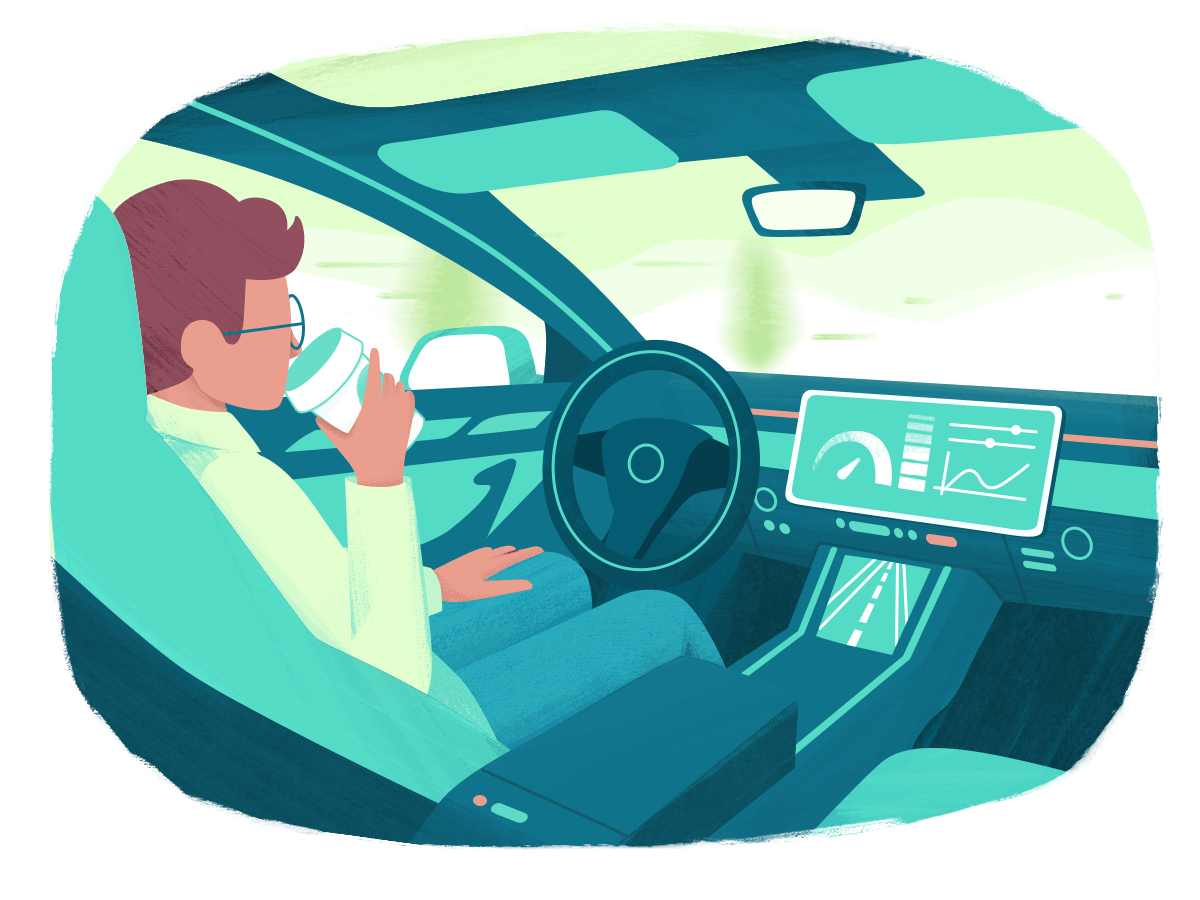
\includegraphics[width=0.50\linewidth]{AV}
	\caption{Concept visualization of autonomous driving. (source: \cite{AV})}
	\label{fig:AV}
\end{figure} 
\newpage

\section{Problem formulation and link with previous studies}
In order to identify the specific comfort preferences of the driver that are quantized by these parameters, the vehicle should be able to learn them by demonstration. \cite{Kuderer2015a}\\
Despite that each driver has its own preferences, they are based on a common notion of comfort where different trade-offs are made. For example, some drivers prefer more aggressive driving than others, which will be manifested in a different set of parameters then which will follow for a defensive driver for the same comfort criteria. The comfort criteria will later in this thesis be translated into an objective function where different weights are used in order to quantify different comfort trade-offs made. This approach is in literature called inverse optimal control because it is learning the objective function of an optimal control problem. The lower the outputted value of this comfort objective by the solution of the optimal control problem, the higher the amount of comfort is attained in the planned path.\\

In order to find comfort criteria which can be used to distinguish different drivers, research about the common notion of comfort is necessary. Passenger surveys in public road transport about carsickness \cite{Turner1999} have identified lateral acceleration as the primarily responsible for motion sickness. It is explained that drive style is a main factor to influence the amount of sickness and it was found that sickness is higher when drivers drove with a higher average magnitude of fore-and-aft and lateral motion. These effect were found far more significant than the effect of vertical vibrations. There is also a consensus reached about the contribution of continuous trajectories to the prevention of motion sickness and the natural feel of paths.\cite{Elbanhawi2015} This means that higher order kinematic variables like accelerations and jerks also should be considered when measuring comfort.\\

\section{Thesis objective}
The goal of this thesis is to build further on the research of learning by demonstration \cite{Kuderer2015a} and to refine this idea in a good working practical application. More concretely the thesis is focussed on the ability to explain driver data and the practical implementation and validation of an algorithm that learns weights of a comfort objective function that is able to capture user specific driving preferences. The learning process is done offline and based on an inverse optimal control approach. The comfort objective will be derived from literature and fitted on individual driver data to produce driver specific parameters. After the different weights are identified, the learned objective can be used to plan paths which can be followed by an autonomous vehicle, making use of an online tracking MPC.\\


To conduct the inverse learning control there is first looked at data generated by simulations where it is assumed that the vehicle is driving on an straight road on high way speed. The maneuver investigated in this thesis is the lane change maneuver as can be seen in Figure \ref{fig:lane_change}. In order to generate data, simulations are done with a non-linear bicycle and a more realistic $15$ dof of freedom Amesim model.


The reader is first given an introduction in the optimal control concepts whereafter in the next chapter the state of the art of comfort modelling is discussed. Next the learning from ideal data is discussed and the learning algorithm is validated by finding back initial chosen weights. After this, the non-linear bicycle model used is substituted by a more complex $15$ degrees of freedom Amesim model. Next there is looked at real expert data generated by a testcar of Siemens. As last an enhancement of the previously used weight update method is proposed and future work to be done is considered.
\begin{figure}[htp]
	\centering
	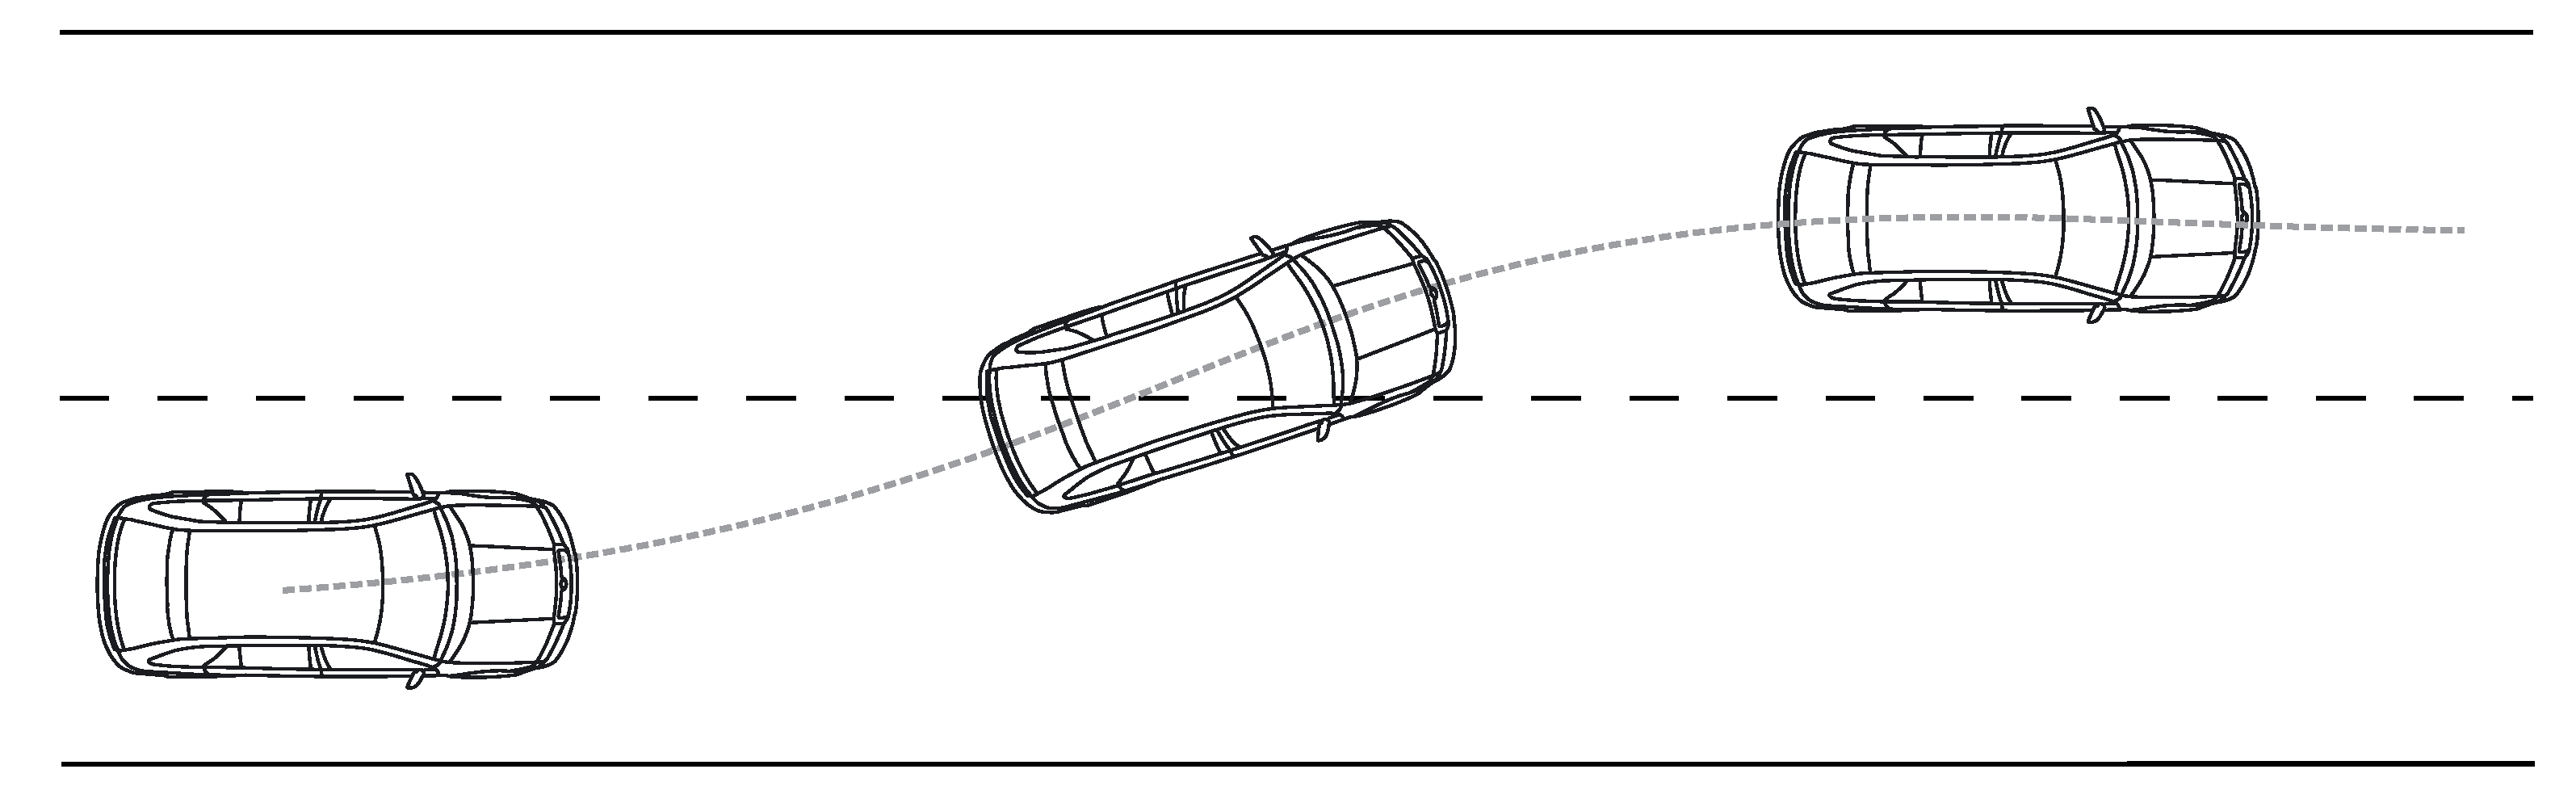
\includegraphics[width=0.8\textwidth]{lane_change.PNG}
	\caption{Example of a lane change which is the investigated maneuver in this thesis.}
	\label{fig:lane_change}
\end{figure}

To be able to make the generated data of high quality an MPC approach with a 15 degree of freedom vehicle model is used. Also in the learning algorithm itself a three degree of freedom non-linear bicycle model is used in order to adequately capture the different kinematic signals e.g. jerks and accelerations. Further there were comparisons made of different methods to learn from multiple datasets. \\

The execution of this research is conducted with the support of "Siemens Digital Industries Software - ADAS R\&D engineering department" located in Leuven which made it possible to preserve a direct link with reality. Software was made available e.g. Simcenter Amesim and the possibility was given to validate the obtained algorithms with real driver data which made it possible to compute more significant results.\\

\textbf{Check of wat verteld werd in de inleiding nog correct is.}

%%% Local Variables: 
%%% mode: latex
%%% TeX-master: "thesis"
%%% End: 
